\section{EODP-TS-E2E. End-to-end test}
\label{sec:e2e}

\subsection{Objective}
The test runs the full chain on a real scene. The modules run in a row and each one reads the outputs of the previous one.
\begin{center}
SGM scene $\rightarrow$ ISM $\rightarrow$ L1B $\rightarrow$ L1C
\end{center}
The scene is a FLEX acquisition over the Pyrenees.
The test checks that the chain runs without errors and that the L1B recovers the input radiance.

\subsection{Inputs and configuration}
The ISM reads the scene in \texttt{EODP-TS-E2E/sgm\_out}. It has 951 lines, 525 columns and 650 wavelengths.
The L1C reads the geolocation in \texttt{EODP-TS-E2E/gm\_out} and the L1B output.
The configuration is the one of \texttt{EODP-TS-E2E/config}. Table~\ref{tab:e2e_config} shows the parameters that change with respect to the unitary tests.
The radiometric errors are disabled, so the L1B does not need the equalization.

\begin{table}[H]
\centering
\caption{E2E configuration. Parameters that differ from the unitary tests.}
\label{tab:e2e_config}
\begin{tabular}{lrr}
\toprule
Parameter & Unitary tests & E2E \\
\midrule
Pixel size $w$ & 30~\textmu m & 42~\textmu m \\
Integration time $t_{int}$ & 6.72~ms & 42.8~ms \\
Pupil diameter $D$ & 0.150~m & 0.07565~m \\
Focal length $f$ & 0.5262~m & 0.2345~m \\
PRNU, dark signal, bad and dead pixels & applied & not applied \\
L1B equalization & yes & no \\
L1B gain VNIR-0 [mW/m$^2$/sr/DN] & 0.0921 & 0.00576 \\
L1B gain VNIR-1 [mW/m$^2$/sr/DN] & 0.0679 & 0.00425 \\
L1B gain VNIR-2 [mW/m$^2$/sr/DN] & 0.0522 & 0.00326 \\
L1B gain VNIR-3 [mW/m$^2$/sr/DN] & 0.0478 & 0.00299 \\
\bottomrule
\end{tabular}
\end{table}

\subsection{Execution}
The script \texttt{harness/EODP-TS-E2E/test\_e2e.py} sets \texttt{EODP\_CONFIG\_DIR} to the E2E configuration and runs the three modules.
The ISM took 195~s, the L1B 11~s and the L1C 61~s. The three modules finished without errors.
As agreed in class, the report shows the L1B results only.

\subsection{Results}

\subsubsection{Altitude}
Figure~\ref{fig:e2e_altitude} shows the variable \texttt{altitude} of \texttt{gm\_out/geolocation.nc} on the map.
The geometry is the same for the four bands, so there is a single plot.
The altitude goes from 131~m to 2972~m. The Pyrenees cross the scene from west to east at about $42.6^\circ$N.

\begin{figure}[H]
\centering
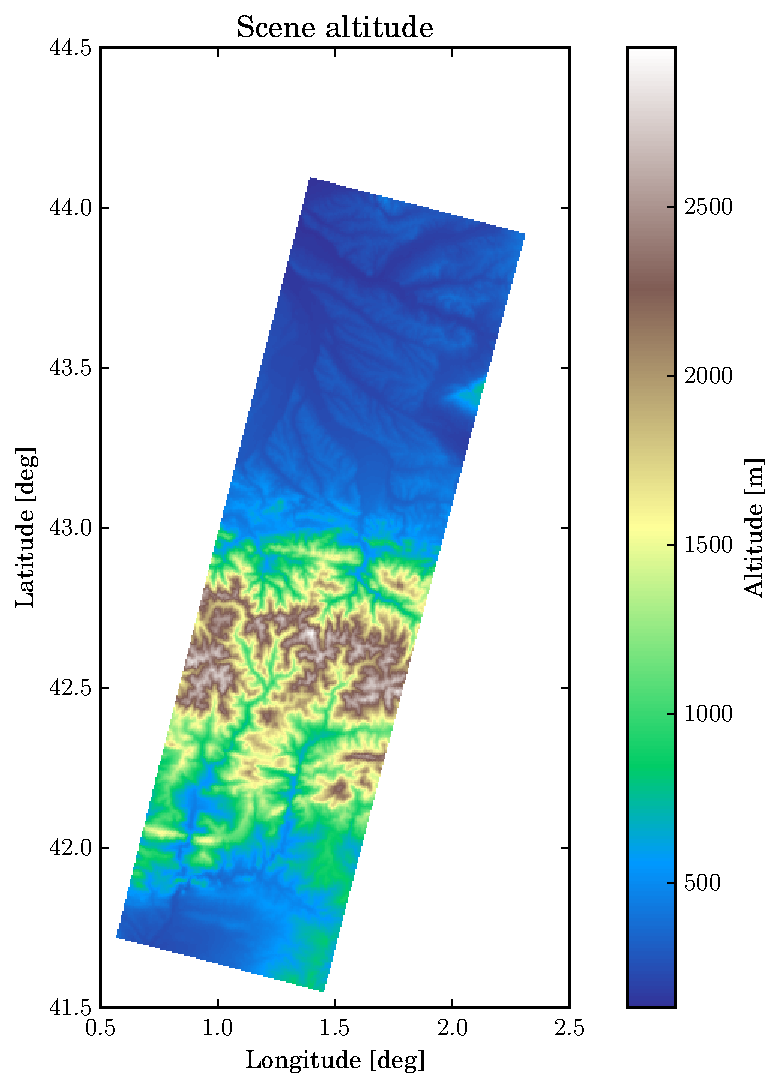
\includegraphics[width=0.7\textwidth]{e2e_altitude}
\caption{E2E. Altitude of the scene.}
\label{fig:e2e_altitude}
\end{figure}

\subsubsection{L1B radiances}
Figures~\ref{fig:e2e_0} to~\ref{fig:e2e_3} show the L1B TOA of each band on the map, with its histogram.
The histograms use bins of 0.1~mW/m$^2$/sr.
The same structures appear in the four bands. The lowest radiances are in the mountains, on the slopes in shadow.
VNIR-0 and VNIR-1 have the highest radiances, up to 13.7~mW/m$^2$/sr. VNIR-2 and VNIR-3 reach 7.1 and 8.5~mW/m$^2$/sr.
The histograms are consistent with the maps. Most pixels are bright and a long tail on the left comes from the shadowed mountain areas.

\begin{figure}[H]
\centering
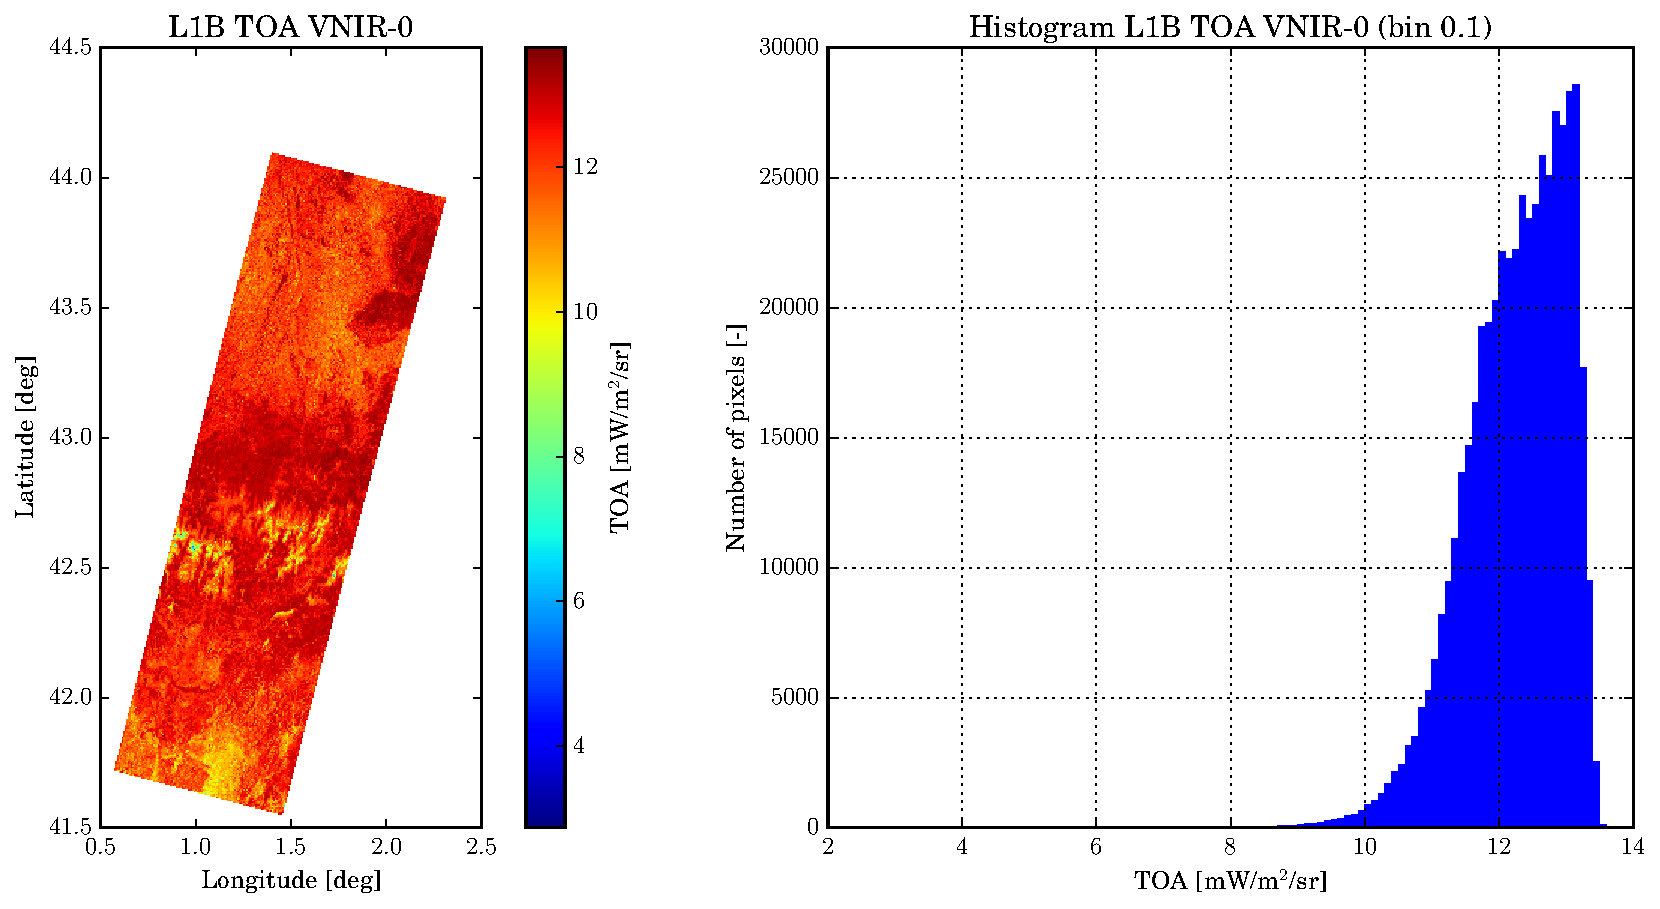
\includegraphics[width=\textwidth]{e2e_l1b_VNIR-0}
\caption{E2E. L1B TOA and histogram, VNIR-0.}
\label{fig:e2e_0}
\end{figure}

\begin{figure}[H]
\centering
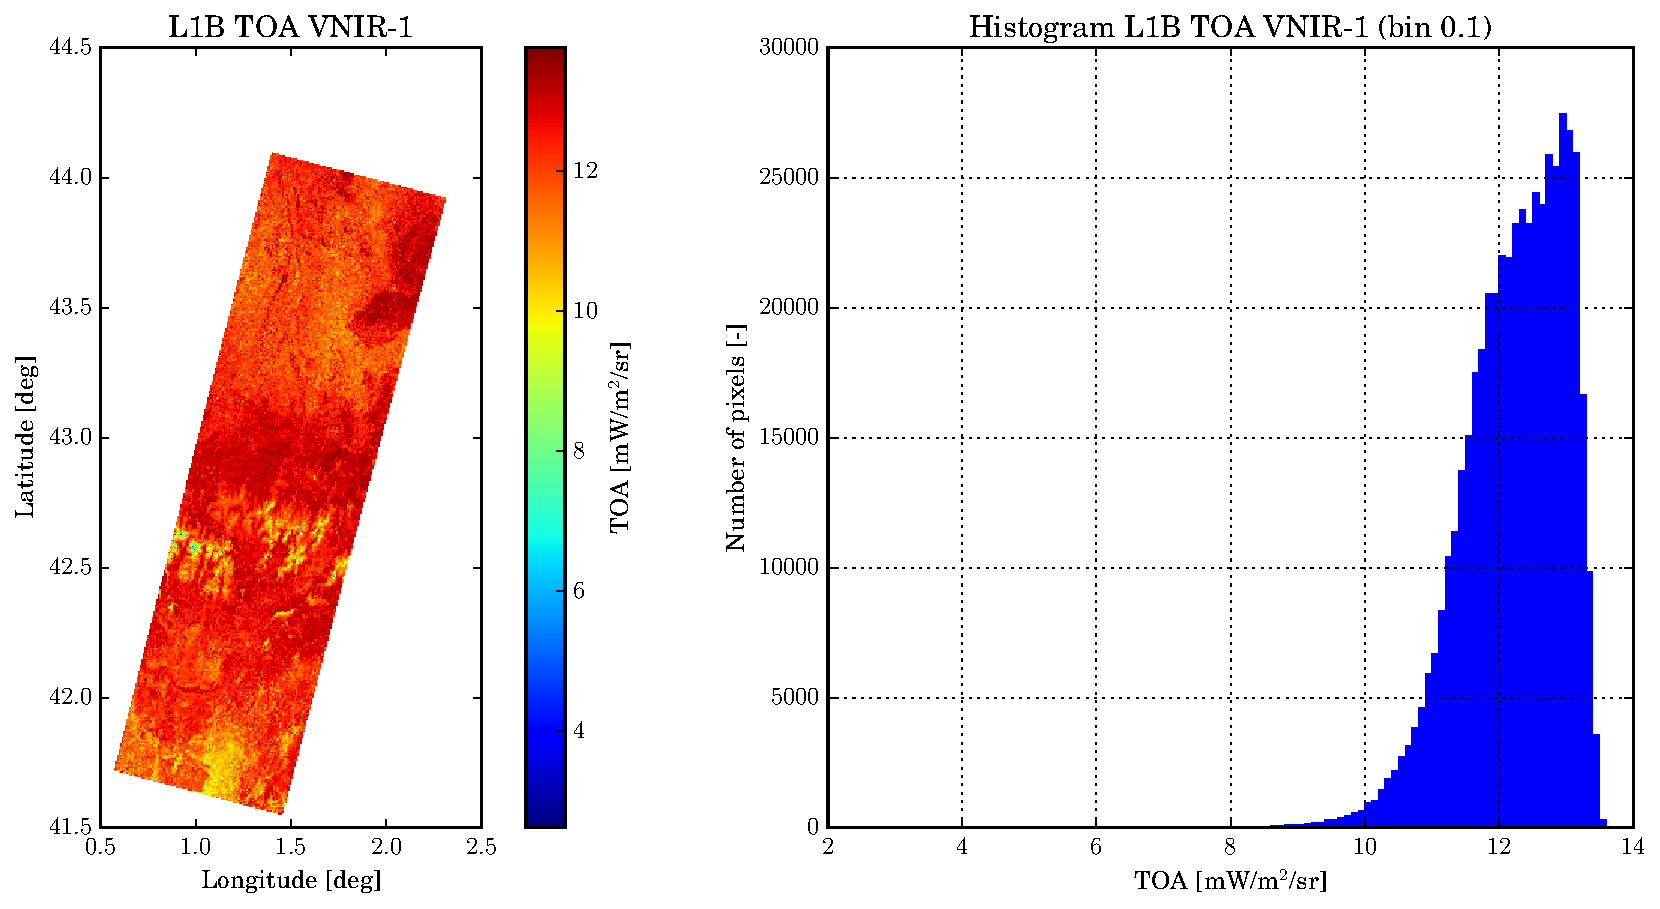
\includegraphics[width=\textwidth]{e2e_l1b_VNIR-1}
\caption{E2E. L1B TOA and histogram, VNIR-1.}
\label{fig:e2e_1}
\end{figure}

\begin{figure}[H]
\centering
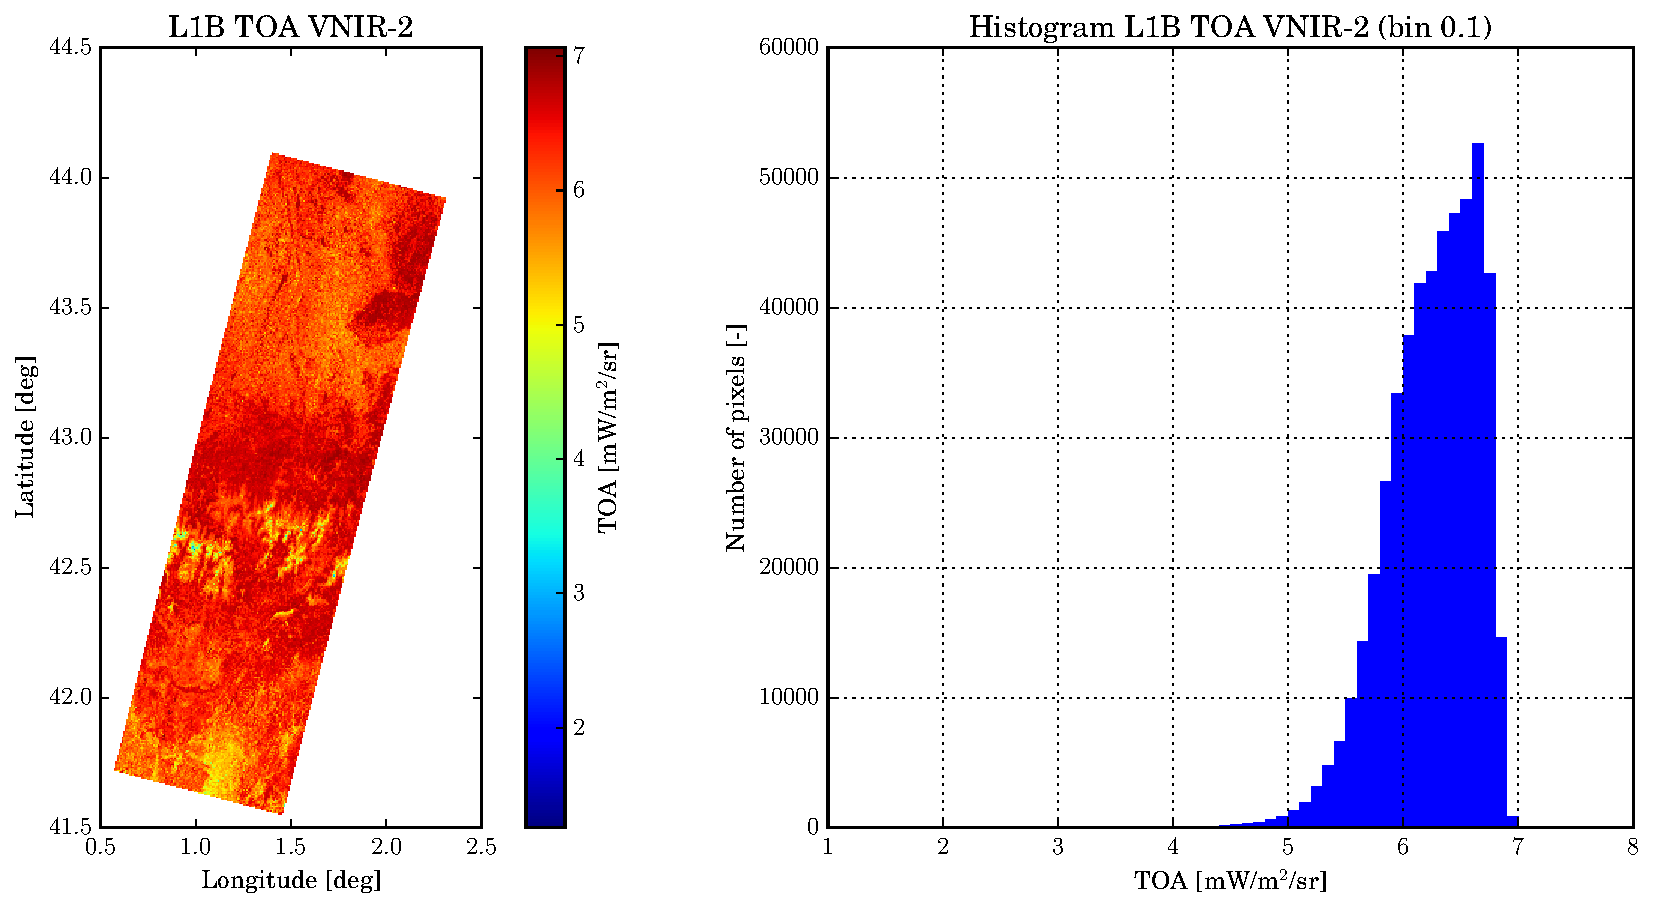
\includegraphics[width=\textwidth]{e2e_l1b_VNIR-2}
\caption{E2E. L1B TOA and histogram, VNIR-2.}
\label{fig:e2e_2}
\end{figure}

\begin{figure}[H]
\centering
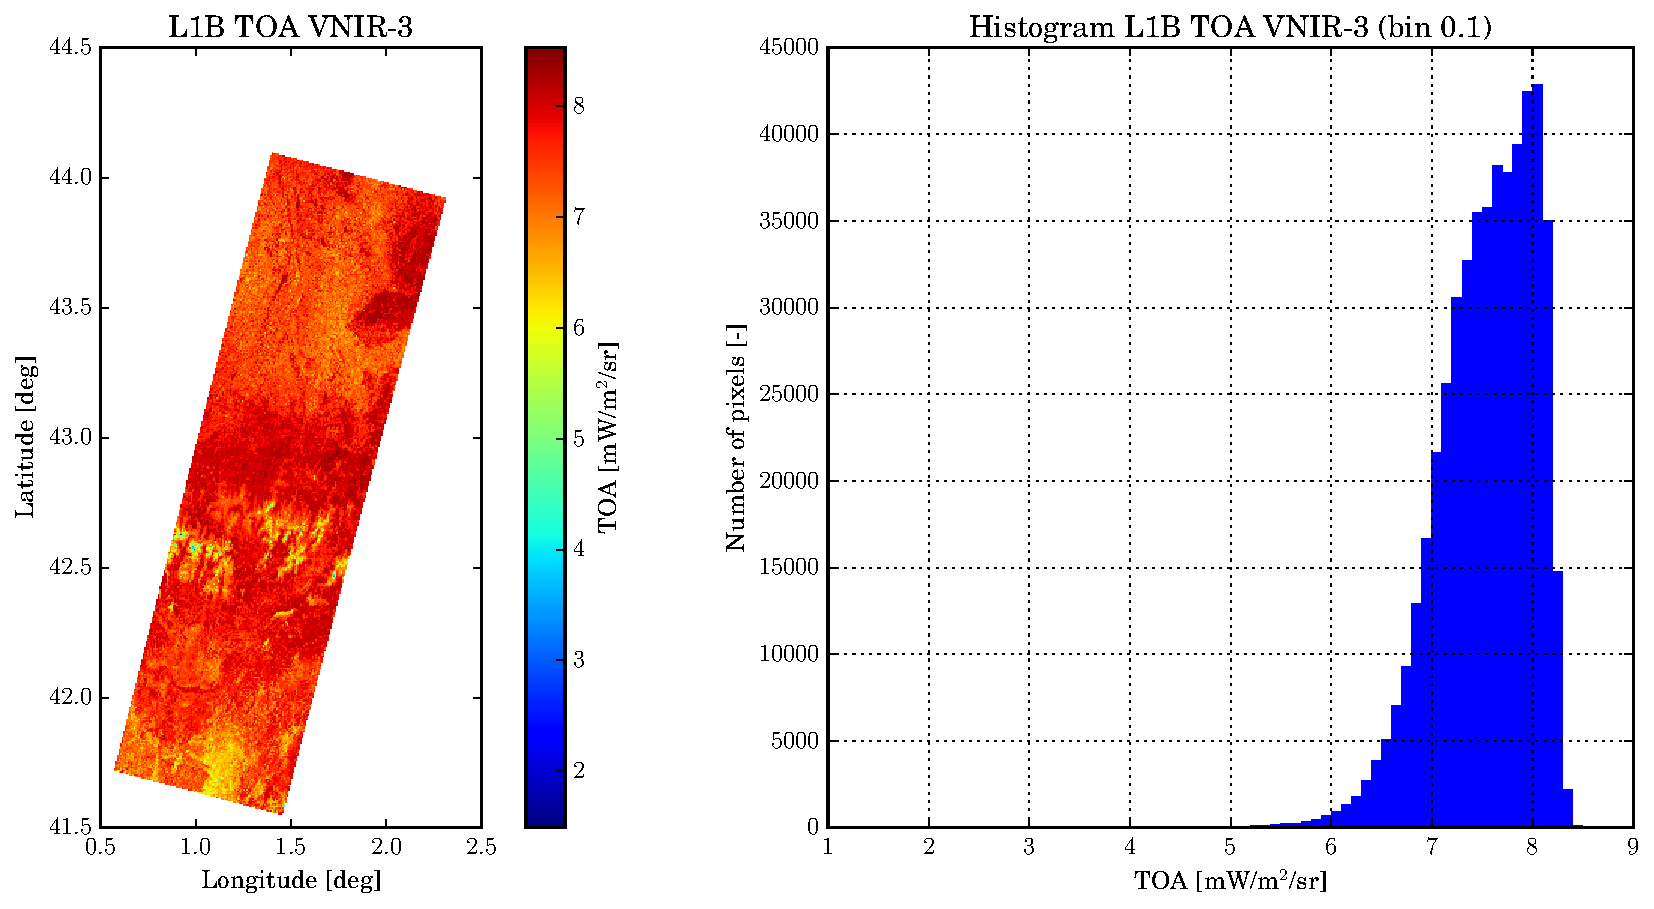
\includegraphics[width=\textwidth]{e2e_l1b_VNIR-3}
\caption{E2E. L1B TOA and histogram, VNIR-3.}
\label{fig:e2e_3}
\end{figure}

\subsubsection{Radiometric consistency}
Without radiometric errors, the L1B should recover the radiance that enters the instrument.
Table~\ref{tab:e2e_radiometry} compares the mean of \texttt{ism\_toa\_isrf} with the mean of \texttt{l1b\_toa}.
The difference is about $-0.02\,\%$ in all the bands. It comes from the MTF and the quantisation.
No pixel is saturated.

\begin{table}[H]
\centering
\caption{E2E. Mean radiance before the instrument and after the L1B [mW/m$^2$/sr].}
\label{tab:e2e_radiometry}
\begin{tabular}{lcccc}
\toprule
Band & Mean ISRF TOA & Mean L1B TOA & Difference [\%] & Saturated [\%] \\
\midrule
VNIR-0 & 12.2554 & 12.2529 & -0.021 & 0.00 \\
VNIR-1 & 12.2348 & 12.2326 & -0.018 & 0.00 \\
VNIR-2 & 6.2529 & 6.2520 & -0.016 & 0.00 \\
VNIR-3 & 7.5464 & 7.5453 & -0.015 & 0.00 \\
\bottomrule
\end{tabular}

\end{table}

As an additional check, the ISM and L1B outputs were compared with the outputs provided with the E2E data.
Table~\ref{tab:e2e_crossval} shows that they are identical within $1.2\times10^{-5}\,\%$.

\begin{longtable}{lccccc}
\caption{E2E. Comparison with the ISM and L1B outputs provided with the E2E data. Maximum relative difference [\%] per band.}\label{tab:e2e_crossval}\\
\toprule
File & VNIR-0 & VNIR-1 & VNIR-2 & VNIR-3 & Result \\
\midrule
\endfirsthead
\toprule
File & VNIR-0 & VNIR-1 & VNIR-2 & VNIR-3 & Result \\
\midrule
\endhead
\texttt{ism\_toa\_isrf\_} & $0$ & $0$ & $0$ & $0$ & Pass \\
\texttt{ism\_toa\_optical\_} & $0$ & $0$ & $0$ & $0$ & Pass \\
\texttt{ism\_toa\_e\_} & $0$ & $0$ & $0$ & $0$ & Pass \\
\texttt{ism\_toa\_detection\_} & $0$ & $0$ & $0$ & $0$ & Pass \\
\texttt{ism\_toa\_} & $0$ & $0$ & $0$ & $0$ & Pass \\
\texttt{l1b\_toa\_} & $1.18\times10^{-5}$ & $1.19\times10^{-5}$ & $1.19\times10^{-5}$ & $1.19\times10^{-5}$ & Pass \\
\bottomrule
\end{longtable}


\subsection{Conclusion}
The chain ISM, L1B and L1C runs without errors on the real scene.
The L1B recovers the mean input radiance within 0.02~\%.
\textbf{EODP-TS-E2E: PASS.}
